
% =========================================================
% PAGE 1: TITLE PAGE 
% =========================================================
\begin{titlepage}
\thispagestyle{empty}

% move header up
\vspace*{-2.5cm}

\noindent
\begin{minipage}[t]{0.45\textwidth}
  \raggedright
  
\includegraphics[height=1.3cm]{HSLU LOGO.png}
\end{minipage}
\hfill
\begin{minipage}[t]{0.45\textwidth}
  \hspace*{1cm}% move right
  
\includegraphics[height=1.2cm]{INFORMATIK.png}
\end{minipage}

    %Hier ein aussagekräftiger Titel und beide Autoren. Eventuell ein illustrierendes Bild.\\ Ansonsten ist diese erste Seite bzw. Frontseite frei gestaltbar.

    % --- This reproduces the big empty space in the Word template ---
    \vspace*{9cm}

    \begin{center}
        {\Huge \textbf{Titel der Transferarbeit}}\\[0.8cm]
        {\Large \textit{Autoren}}\\[1.5cm]
        \vfill
    \end{center}
\end{titlepage}

% =========================================================
% PAGE 2: FORMAL INFO + DECLARATION + LINK 
% =========================================================
\newpage
\thispagestyle{empty}

\begin{center}
{\Large \textbf{Transferarbeit an der Hochschule Luzern – Informatik}}
\end{center}

\vspace{1cm}

\noindent
\textbf{Titel:} 

\vspace{0.6cm}

\noindent
\textbf{Teilnehmerin/Teilnehmer:} 

\vspace{0.6cm}

\noindent
\textbf{Teilnehmerin/Teilnehmer:} 

\vspace{0.8cm}

\noindent
\textbf{Programm:} CAS Software Architecture

\vspace{0.6cm}

\noindent
\textbf{Zeitraum:}

\vspace{0.8cm}

\noindent
\textbf{Programmleitung:} Prof.\ Dr.\ habil.\ Jana Koehler, Dr.\ Stefan Bischoff

\vspace{0.6cm}

\noindent
\textbf{Betreuung/Referat:} 

\vspace{1.2cm}

\noindent
\textbf{Codierung / Klassifizierung der Arbeit:}

\vspace{0.4cm}

\noindent
\checkedbox\ Öffentlich (Normalfall)

\noindent
\uncheckedbox\ Vertraulich

\vspace{1.2cm}

\noindent
\textbf{Eidesstattliche Erklärung}

\vspace{0.4cm}

\noindent
Ich erkläre hiermit, dass ich/wir die vorliegende Arbeit selbständig und ohne unerlaubte fremde Hilfe angefertigt haben, alle verwendeten Quellen, Literatur und andere Hilfsmittel angegeben haben, wörtlich oder inhaltlich entnommene Stellen als solche kenntlich gemacht haben, das Vertraulichkeitsinteresse des Auftraggebers wahren und die Urheberrechtsbestimmungen der Hochschule Luzern respektieren werden.

\vspace{1.4cm}

\noindent
Ort / Datum, Unterschrift \hspace{0.7em}\rule{10.2cm}{0.4pt}

\vspace{1.0cm}

\noindent
Ort / Datum, Unterschrift \hspace{0.7em}\rule{10.2cm}{0.4pt}

\vspace{1.6cm}

\noindent
Geistiges Eigentum gemäss der
\href{https://srl.lu.ch/app/de/texts_of_law/521/versions/3884}{Studienordnung}
für die Ausbildung an der Hochschule Luzern, FH Zentralschweiz

% =========================================================
% PREFACE TEXT 
% =========================================================
\newpage
\pagenumbering{arabic}

\noindent
% Das folgende Template ist im Wesentlichen von arc42 übernommen. Bitte passt es an entsprechend Eurer Arbeitsschwerpunkte, unseren Pflichtinhalten und den Methoden, die wir im Kurs verwenden. Ich habe auch noch einige zusätzliche Kommentare hinzugefügt, die erklären was wir in den einzelnen Kapiteln an Inhalten gerne sehen würden. Seitenzahlen sind eingefügt und in der Fusszeile sichtbar. Sollten hier Probleme bei Euch auftreten, schaut in Word unter Einfügen > Fusszeile bearbeiten und stellt sicher, dass «Mit vorheriger verknüpfen» aktiviert ist. Ihr könnt gerne die Seitenzahlen auch an einer anderen Position platzieren, z.B. in der Kopfzeile, wenn es Euch besser gefällt.

\vspace{1cm}

% =========================================================
% TABLE OF CONTENTS / LIST OF FIGURES
% =========================================================
\tableofcontents
\newpage

\listoffigures
\newpage

% -------------------------------------------------
% NOTE ON FIGURES & REFERENCES 
% -------------------------------------------------
% Use captions for figures in a way such that they are automatically maintained by LaTeX.
% In Word this is "Referenzen > Beschriftung einfügen".
% In LaTeX you do this with:
%   \begin{figure} ... \caption{...}\label{fig:xyz}\end{figure}
% and refer to it with:
%   Figure~\ref{fig:xyz}
%
% Hier ein Beispiel für eine Referenz, die dann auch automatisch aktualisiert:
% In Figure~\ref{fig:iso25010}, we discuss …
% (In Word: Einfügen > Querverweis)
%
% Example figure block (upload the image file into Overleaf):
% \begin{figure}[H]
%   \centering
%   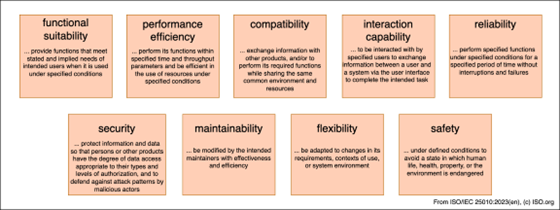
\includegraphics[width=0.9\textwidth]{iso25010.png}
%   \caption{Overview on ISO 25010}
%   \label{fig:iso25010}
% \end{figure}

